\chapter{Wyniki i testy wydajnościowe}
\label{chap:research}

Ten rozdział zawiera zrzuty ekranu pokazujące wyrenderowane przykładowe sceny oraz testy wydajnościowe mierzące wydajność implementacji cieniowania odroczonego.


\section{Przykładowe sceny}

Używane sceny zostały przygotowane na podstawie zebranych przez Khronos w repozytorium \cite{GLTFSAMPLEMODELS} następujących przykładowych modelów glTF przedstawiających:
\begin{itemize}
	\item \textit{MetalRoughSpheres}: różne wartości metalu i chropowatości materiałów używając sfer, patrz rys. \ref{screenshot_metalroughspheres};
	\item \textit{DamagedHelmet}: uszkodzony w walce hełm sci-fi, patrz rys. \ref{screenshot_damagedhelmet};
	\item \textit{Sponza}: wnętrze budynku inspirowane pałacem Sponza, często używane do testowania oświetlenia, patrz rys. \ref{screenshot_sponza}.
\end{itemize}

\begin{figure}[!htb]
	\centering
	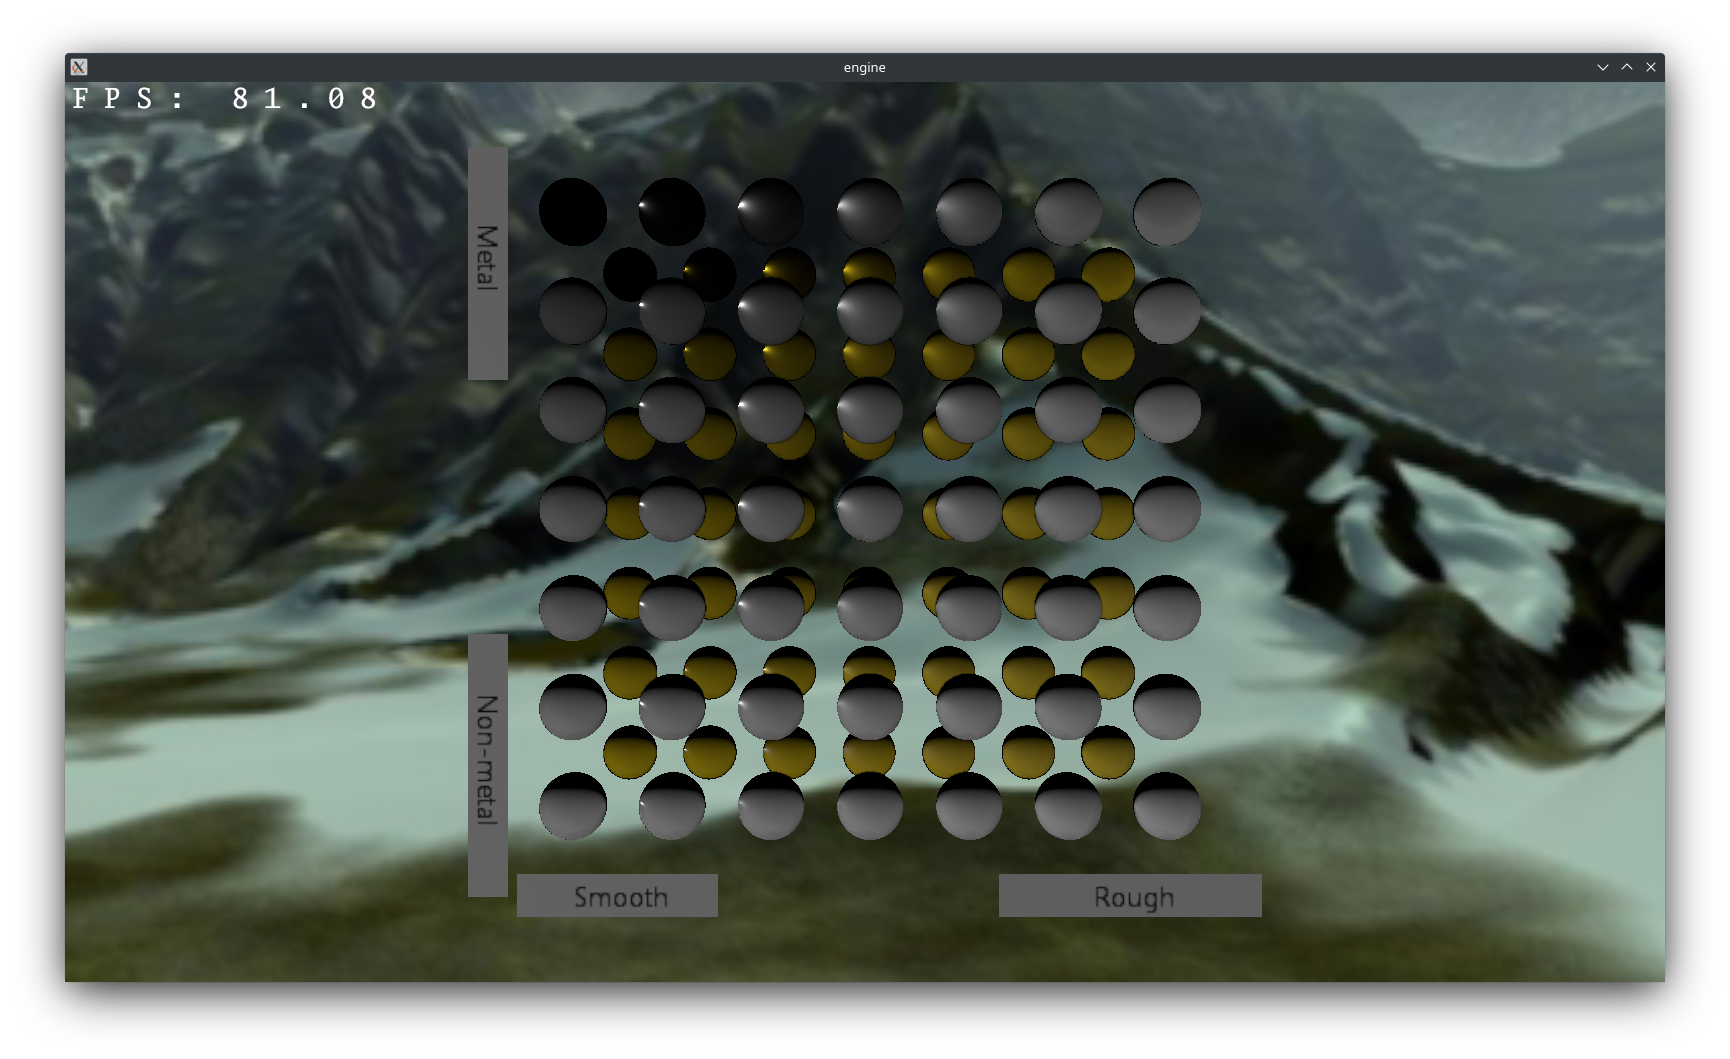
\includegraphics[width=0.8\textwidth]{images/render_metalroughspheres.png}
	\caption{Wynik renderowania sceny MetalRoughSpheres (opracowanie własne)}
	\label{screenshot_metalroughspheres}
\end{figure}

\begin{figure}[!htb]
	\centering
	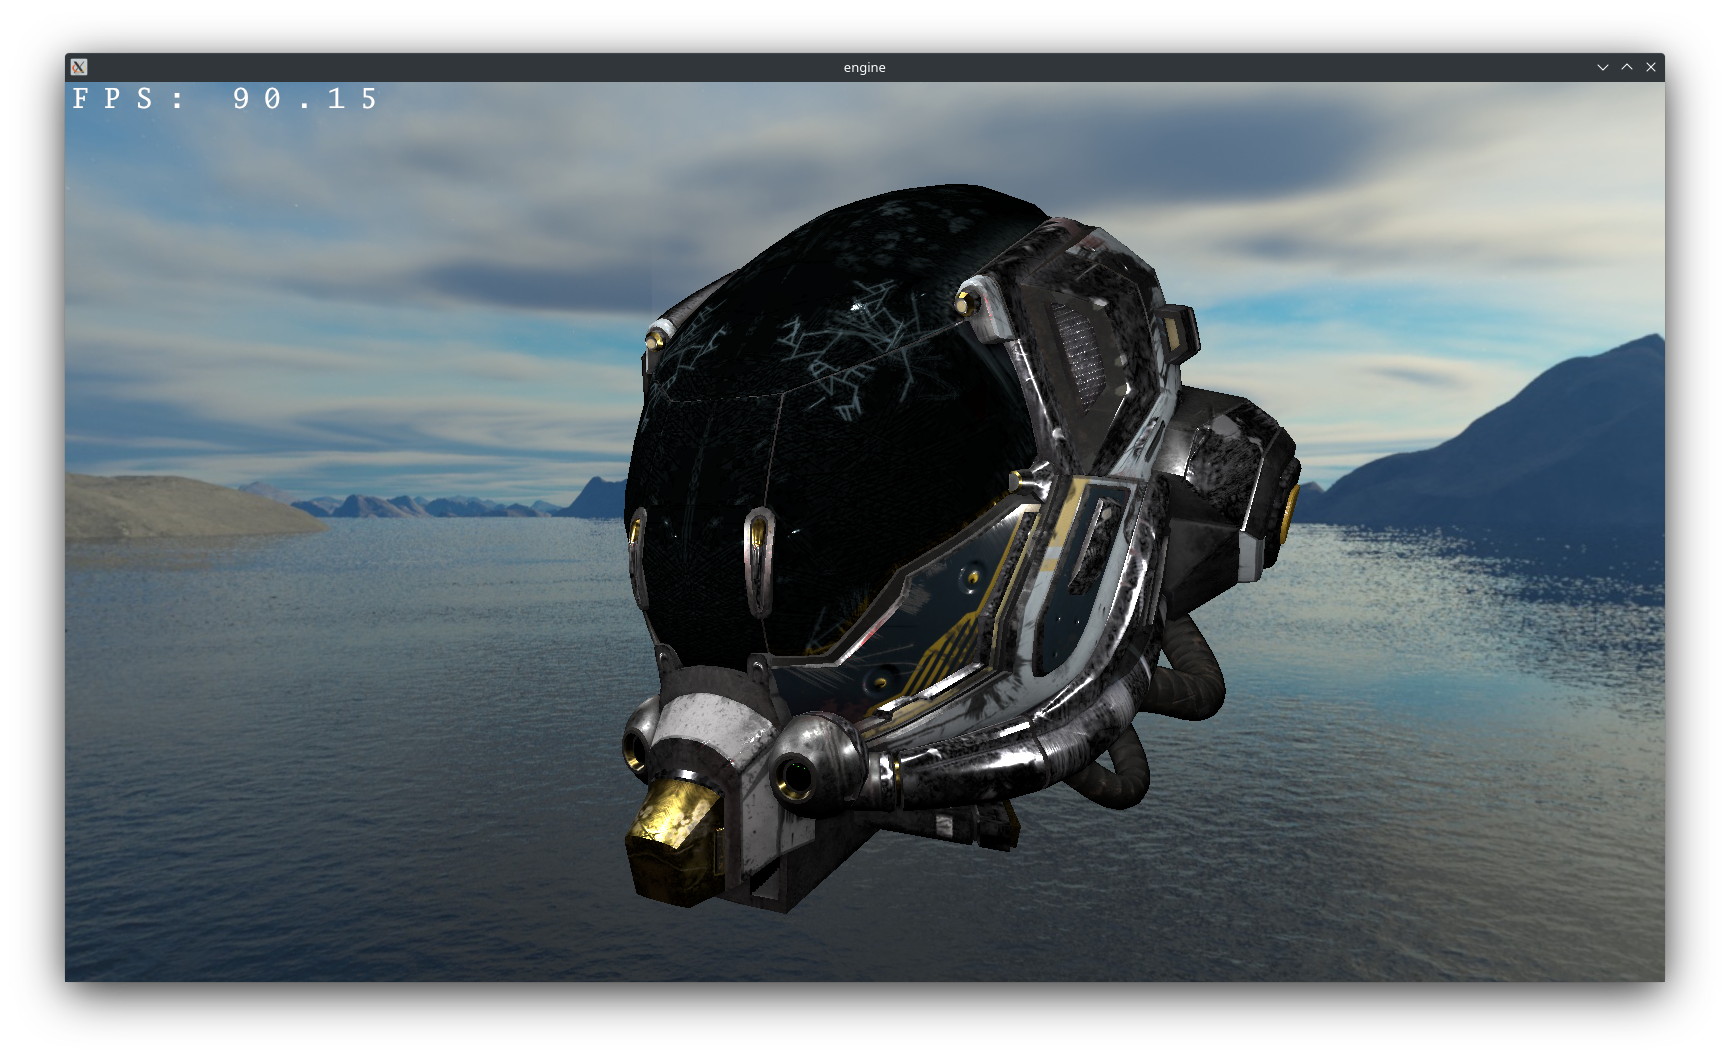
\includegraphics[width=0.8\textwidth]{images/render_damagedhelmet.png}
	\caption{Wynik renderowania sceny DamagedHelmet (opracowanie własne)}
	\label{screenshot_damagedhelmet}
\end{figure}

\begin{figure}[!htb]
	\centering
	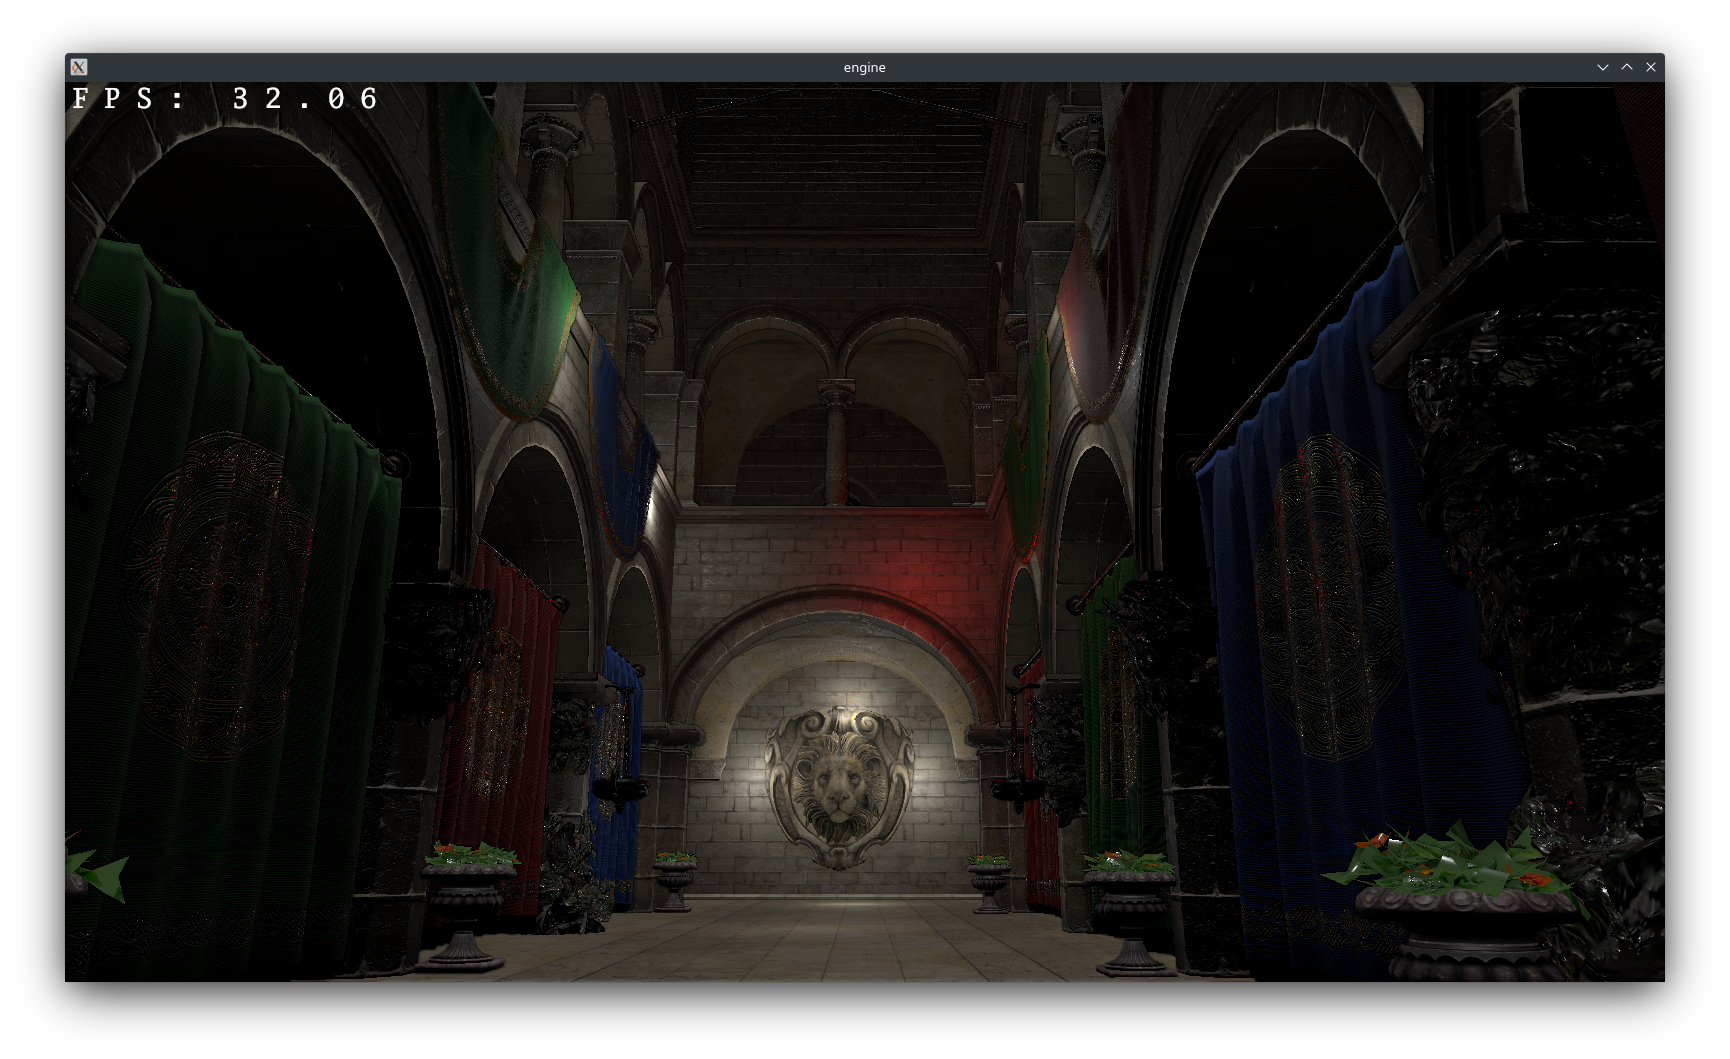
\includegraphics[width=0.8\textwidth]{images/render_sponza.png}
	\caption{Wynik renderowania sceny Sponza (opracowanie własne)}
	\label{screenshot_sponza}
\end{figure}

\section{Testy wydajnościowe}

Zbadano wydajność implementacji cieniowania odroczonego poprzez renderowania sceny Sponza w 10 eksperymentach spowodowanych zmianą następujących zmiennych:
\begin{itemize}
	\item rozdzielczości okna: 640x480, 1600x900;
	\item liczby świateł punktowych: 1, 30, 75, 10, 100.
\end{itemize}

Zmierzono liczbę klatek na sekundę poprzez obserwację maksymalnych i minimalnych wartości wyświetlanych podczas działania programu licznik FPS silnika w lewym górnym rogu okna, które są zbliżone do wartościi reportowanych przez warstwę \textit{VK\_LAYER\_MESA\_overlay}.

Zmierzono udział poszczególnych etapów potoku graficznego podczas wykonywania poleceń rysowania poprzez przechwycenie 10 klatki aplikacji narzędziem RenderDoc i zbadanie liczników wydajności.
Po porównianiu wartości liczników wydajności z różnych eksperymentów okazało się, że największe zmierzone zmiany, które nie mogą być wytłumaczone błędem przypadkowym spowodowanym nieprzewidywalnością działania potoku graficznego GPU, zachodzą dla polecenia rysowania w przebiegu oświetlenia G-bufora dla następujących liczników wydajności oferowanych przez GPU firmy Intel:
\begin{itemize}
	\item \textit{L3 Shader Throughput (bytes)}: całkowita liczba bajtów pamięci GPU przesyłanych pomiędzy shaderami a pamięcią podręczną L3;
	\item \textit{Shader Memory Accesses}: całkowita liczba operacji dostępu do pamięci buforów w shaderach;
	\item \textit{Samplers Busy (\%)}: procent czasu spędzony na próbkowaniu obrazów.
\end{itemize}

Wyniki pomiarów wydajności prezentuje tabela \ref{results_sponza}.

\begin{table}[!ht]
	\centering
	\begin{tabular}{ |p{2cm}|p{1.1cm}||p{0.7cm}|p{0.7cm}|p{1.8cm}|p{1.7cm}|p{1.6cm}|}
		\hline
		Rozdzielczość okna & Liczba świateł & FPS Min & FPS Max & L3 Shader Throughput (bytes) & Shader Memory Accesses & Samplers Busy (\%) \\
		\hline \hline
		640x480 & 1 & 101 & 129 & 19685376 & 307584 & 97.3006 \\
		\hline 
		640x480 & 10 & 86 & 104 & 68837824 & 1075591 & 88.82873 \\
		\hline 
		640x480 & 30 & 70 & 79  & 179433088 & 2803642 & 50.89936 \\
		\hline 
		640x480 & 75 & 46 & 48 & 428882496 & 6701289 & 26.02086 \\
		\hline 
		640x480 & 100 & 37  & 40 & 566511168 & 8851737 & 20.69141 \\
		\hline 	\hline 
		1600x900 & 1 & 37  & 42 & 92281664 & 1441901 & 99.45081 \\
		\hline 
		1600x900 & 10 & 29  & 31 & 322695168 & 5042112 & 89.91253 \\
		\hline 
		1600x900 & 30 & 19 & 21 & 841100544 & 13142196 & 57.64096 \\
		\hline 
		1600x900 & 75 & 11 & 12 & 2010387968 & 31412312 & 26.82165 \\
		\hline 
		1600x900 & 100 & 9  & 10 & 2655508160 & 41492315 & 21.54303 \\
		\hline
	\end{tabular}
	\caption{Wyniki pomiarów dla sceny Sponza (opracowanie własne)} 
	\label{results_sponza}
\end{table}


// HIRO interpretacja
